\documentclass[12pt,letterpaper]{article}
\usepackage[T1]{fontenc}
\usepackage{anysize}
\usepackage{tikz}
\usepackage{amssymb}
\usepackage{comment}
\usepackage{graphicx}
\usepackage{amssymb}
\usepackage{algpseudocode}

\setlength{\parindent}{0cm}
\setlength{\parskip}{1em}

\newcommand{\contradiction}{%

\begin{tikzpicture}[rotate=45,x=0.5ex,y=0.5ex]
\draw[line width=.2ex] (0,2) -- (3,2) (0,1) -- (3,1) (1,3) -- (1,0) (2,3) -- (2,0);
\end{tikzpicture}
}

\marginsize{2cm}{2cm}{1cm}{1cm}

\begin{document}

\begin{titlepage}
    \vspace*{4cm}
    {\huge \center
        CS 325 Traveling Salesman Report\\[1cm]
    }
    \center
    {\large
        Group 3

        Date: \today

    \textbf{Contributors:}
    Cezary Wojcik,
    Sean McGlothlin,
    Matthew Eilertson
    }

\end{titlepage}

\section*{Introduction}

The Travelling Salesman Problem (TSP) is a classic problem - given a set of cities and distances between those cities, find the shortest possible loop that visits every city. The TSP is an NP-Hard problem that has a brute force running time of $O(n!)$, which is obviously fairly inefficient. Instead of finding an optimal solution, we will be finding "good enough" solutions that are found much more quickly.

Our TSP algorithm finds "good" solutions through a combination of random permutations and divide and conquer. The cities are divided into groups on a grid recursively until groups have at most 6 cities, and then $n^S$ (where $n$ is the number of cities in the group and $S$ is our "speed constant") random solutions are generated in each isolated grid. Once the best solutions are found, the groups are joined in the same fashion.

\section*{Random Permutations}

A core part of our algorithm for the TSP is to simply create a random order of cities to be visited. While random luck is not always a good idea, we can reduce the likelihood of bad solutions by running lots of random solutions and selecting the one that has the shortest path. In this implementation, each newly randomized path is compared to the minimum path discovered so far. If it is shorter, then the new path becomes the minimum path, and the old one is discarded. This method is more effective on smaller sets of cities since there are fewer permutations of cities. Larger sets have much more permutations, so the odds of finding suboptimal paths are much higher.

This idea was, to some extent, inspired by Group 18's approach using random neighbor inclusion. In their approach, they took a small set of close cities, connected them, and then added random cities to the loop until all the cities are included. They would then run this algorithm multiple times and keep the shortest path found. We decided to change their idea by removing the requirement of finding a close set of cities first, which could be slow. Instead, we create many more permutations of cities and keep track of the best path.

\section*{Divide and Conquer}

One of the major difficulties of the TSP is that optimal solution algorithms quickly become more difficult to find as the number of cities increase ($n!$ grows quickly). Applying only the idea of random permutations to a large set of cities isn't plausible because it would require an even larger number of random permutations. By applying a divide and conquer method, we can process larger sets of cities faster.

As the algorithm reads in the cities of the TSP, we create an initial grid of $5 \times 5$ to separate the cities into smaller groups. However, the cities may be densely grouped, so if any individual block contains more than a specific threshold, $T$, then we divide that block into another $5 \times 5$ grid. Subdivisions continue recursively until the threshold is satisfied. This method makes use of the fact that the random permutations method is far more effective with smaller sets of cities.

\section*{Divide and Conquer With Randomized Assembly}

Once our algorithm has divided the problem into a number of smaller subproblems, the randomized path trials begin in each block. We will calculate $n^S$ random paths, where $n$ is the number of cities in a given grid block. Next, we take the minimum path found and return that path to be connected to the other shortest paths found in the other blocks. Once all of the shortest paths have been found, randomized path trials are again used to connect the blocks to other blocks by treating the subpaths as individual cities, and then those are in turn connected to even larger blocks until all the cities are connected in a tour.

We used $S=3$ because in our testing, it seemed as though 3 is the best compromise between decent results and fast execution time. Below is a graph that shows these variables for example input 1 (76 cities). We can see that the average (out of 100 tests) result (path length) decreases as $S$ increases, but after $S=3$, we don't get as much benefit from the higher execution time.

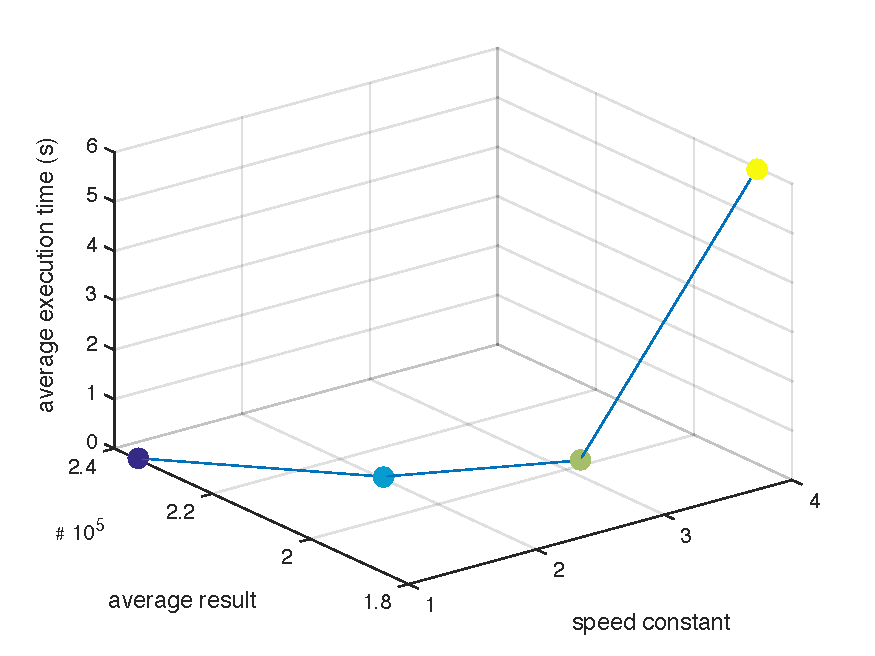
\includegraphics[height=190pt]{fig1.pdf}

\section*{Shortest Path Improvability}

We wrote our code in a way such that our "pathfinder" function can be replaced with any function that can determine the shortest path of a graph, and the code will still work just the same using our divide and conquer pattern. It would likely be fairly simple to find some MST library or shortest path implementation (such as Bor\r{u}vka's Algorithm, as we discussed in our presentation) and use that in place of the pathfinder function we wrote.

\newpage

\end{document}
